\documentclass{article}
\usepackage[utf8]{inputenc}
\usepackage{graphicx}
\usepackage{float}
\usepackage{hyperref}
\usepackage{amssymb}
\usepackage{listings}
\usepackage[parfill]{parskip}
\usepackage[rmargin=0.6in,lmargin=0.6in,tmargin=0.7in, bmargin=0.7in]{geometry}

\title{CUDA accelerated CSR Matrix Conjugate Gradient Method}
\author{Filip Čacký}
\date{2023\\ April}

\begin{document}

\maketitle

\section{Abstract}
The focus of this term paper is the implementation of a CUDA accelerated CSR sparse matrix
conjugate gradient method for solving systems of linear equations.

The implementation details of a CPU version are discussed first,
followed by implementations of CUDA kernels for the required mathematical operations
accompanied by profiler outputs.
Finally both versions are benchmarked on several different equations and compared.

The CUDA accelerated version achieved a speedup of up to 10x when compared to the parallelized CPU version.

\section{Problem definition}
The conjugate gradient method (CGM) is an iterative method for solving systems of linear equations $Ax = b$
where $A$ is an $n\times n$ symmetric, positively-definite real matrix \cite{wiki_cgm}.

A pseudo-code implementation of the algorithm is depicted in Figure \ref{code:cgm_pseudo}.

\begin{figure}[H]
\begin{lstlisting}[language=Python,mathescape=true]

def cgm(A, b, max_iterations, permissible_error):
  $k := 0$
  $r_k := b - A * x_k$
  $p_k := r_k$

  while $k$ <= max_it and $|r_k|_2$ < permissible_error: 
    $a_k := \frac{r_k^Tr_k}{p_k^TAp_k}$
    $x_{k+1} := x_k + a_kp_k$
    $r_{k+1} := r_k + a_kAp_k$
    $b_k := \frac{r_{k+1}^Tr_{k+1}}{r_k^Tr_k}$
    $p_{k+1} := r_{k+1} + b_kp_k$

    $k := k + 1$Upon analyzing the warp stall sampling, it becomes evident that the majority of time spent within the kernel is attributed to global memory access, which proves to be challenging to optimize due to the inherent characteristics of the algorithm.

  return $x_k$

\end{lstlisting}
\caption{Conjugate gradient method pseudo-code \cite{wiki_cgm}}
\label{code:cgm_pseudo}
\end{figure}

The following operations have to be implemented.

\begin{itemize}
  \item $A \cdot v$
  \item $v \cdot u$
  \item $v + \alpha v$
  \item $v - \alpha v$
\end{itemize}

Where $A$ is a matrix, $v$ and $u$ are vectors of valid length and $\alpha$ is a scalar.

\section{Sparse matrices}
A sparse matrix is a matrix in which most elements are zero.
The number of zero valued elements in the matrix divided by the total number of elements
is referred to as sparsity of the matrix.
Similarly, the number of non-zero valued elements in the matrix divided by the total number
of elements is referred to as density of the matrix \cite{wiki_csr}.

This term paper considers only Compressed Sparse Row (CSR) matrices.
A CSR matrix is represented by three vectors of values, instead of
a row or column-major value storage format used in dense matrices.

The focus of this term paper is solely on implementing CGM for Compressed Sparse Row (CSR) matrices.
In a CSR matrix, the non-zero elements of the matrix are stored along with their row and column indices.

The CSR matrix format is characterized by three arrays:
\begin{itemize}
  \item non-zero values
  \item column indices corresponding to each value
  \item value vector indices corresponding to the first non-zero value in each row
\end{itemize}

This storage approach has several advantages such as a lower storage or memory footprint
and faster matrix-vector dot product operations for matrices with a large sparsity.

\section{Implementation details}
The CPU version was implemented with the use of the OpenMP parallelization toolkit,
utilizing parallel for and parallel reductions for all required operations.

The CUDA accelerated version was implemented with the aid of the
NVIDIA Thrust parallel algorithms library \footnote{https://github.com/NVIDIA/thrust}.
At first, all operations were implemented with the functional Thrust interface with custom
functors. This was later rewritten in pure CUDA due to a relatively large overhead
and the Thrust library was kept only for memory management.

\subsection{Vector dot product}
The first iteration of the vector dot product cuda kernel is depicted in Figure \ref{code:vdot_pseudo}.
This version utilizes one thread per vector element and performs a warp shuffle
to reduce each warp before atomically summing the warp results.
The warp shuffle is used in order to reduce the amount of required atomic operations.
Launching one thread per vector element may be unwanted in scenarios 
when several kernels need to be run at the same time,
it makes any debugging of the code more difficult and makes kernel launching error prone.

An improvement was made using a grid-stride loop recommended on the NVIDIA developer blog
\footnote{https://developer.nvidia.com/blog/cuda-pro-tip-write-flexible-kernels-grid-stride-loops/}.
The improved pseudo code is depicted in Figure \ref{code:vdot_pseudo_stride}.

\begin{figure}[H]
\begin{lstlisting}[language=Python,mathescape=true]

def dot(v, u, result):
  threadId := blockDim.x * blockIdx.x + threadIdx.x
  lane := threadId % cuWarpSize
  mask := cuWarpActive(threadId < size(v))
  if threadId >= size(v):
    return

  local_res := first[threadId] * second[threadId];
  local_res = warpReduce(local_res, mask);
  if (lane == 0)
    atomicAdd(result, local_res);

\end{lstlisting}
\caption{Basic vector dot product pseudo-code}
\label{code:vdot_pseudo}
\end{figure}

\begin{figure}[H]
\begin{lstlisting}[language=Python,mathescape=true]

def dot(v, u, result):
  threadId := blockDim.x * blockIdx.x + threadIdx.x
  threadCnt := blockDim.x * gridDim.x;
  lane := threadId % cuWarpSize

  idx := threadId;
  mask := cuWarpActive(threadId < size(v))

  while idx < size:
    local_res = first[idx] * second[idx];
    local_res = cuWarpReduce(local_res, mask);
    if (lane == 0)
      atomicAdd(result, local_res);

    idx += threadCnt;
    mask = cuWarpActive(idx < size(v))

\end{lstlisting}
\caption{Vector dot product with stride pseudo-code}
\label{code:vdot_pseudo_stride}
\end{figure}

\subsection{CSR matrix-vector dot product}
The first implemented CSR matrix-vector dot product kernel
uses a single thread for each row in the matrix,
making it most effective for matrices with a low average count of non-zero values per row.

The pseudocode of this approach is depicted in Figure \ref{code:csrv_1thread}.
The implementation uses a grid stride loop, this is ommited for the sake of brevity.

\begin{figure}[H]
\begin{lstlisting}[language=Python,mathescape=true]

def dot(A, x, result):
  threadId := blockDim.x * blockIdx.x + threadIdx.x;

  if threadId >= height(A):
    return

  segment_begin := A.row_ptr[threadId];
  segment_end := A.row_ptr[threadId + 1];
  
  result = 0;
  
  for idx in range(segment_begin, segment_end):
    result += x[A.col_idx[idx]] * A.values[idx]
  
  output[row] = result;

\end{lstlisting}
\caption{CSR matrix vector pseudo-code 1 thread per row}
\label{code:csrv_1thread}
\end{figure}

The second kernel uses a one warp (i.e. 32 threads) for each row in the matrix,
making it most effective for matrices with a larger count of non-zero values per row.
Each row operation follows a similar pattern as the vector dot product, involving a warp shuffle followed by an atomic sum.
The pseudocode is depicted in Figure \ref{code:csrv_warp}.
The implementation uses a warp stride loop in order to allow arbitrary kernel launches.

\begin{figure}[H]
\begin{lstlisting}[language=Python,mathescape=true]

def dot(A, x, result):
  threadId := blockDim.x * blockIdx.x + threadIdx.x;
  warpId := threadId / cuWarpSize;
  lane := threadId % cuWarpSize;

  segment_begin := A.row_ptr[warpId];
  segment_end := A.row_ptr[warpId + 1];

  for idx in range(segment_begin + lane, segment_end, cuWarpSize):
    result += vector_data[col_idx[idx]] * mx_data[idx];

  result = cuWarpReduce(result, cuFullMask);

  if (lane == 0)
    output[warpId] = result;

\end{lstlisting}
\caption{CSR matrix vector pseudo-code 1 warp per row}
\label{code:csrv_warp}
\end{figure}

\section{Performance analysis and optimizations}

To identify any sections of the code that requires optimizations,
we execute the program using NVIDIA Nsight Systems profiler.

In Figure \ref{img:nsight_cuda_api},
the runtime of CUDA API calls is depicted.
The profiled program underwent 10,000 iterations,
with cudaMemcpy being invoked approximately 20,000 times (twice per iteration for each dot product in the algorithm).
While it takes up ~82\% of the CUDA api running time, it is impossible to be reduced.
There are no operations to be overlayed with it with an async call and the result is immediately required.

cudaMalloc and cudaFree are invoked an equal number of times and account for roughly 7\% of the overall runtime,
removing the excess allocations is quite an easy optimization to make.

\begin{figure}[H]
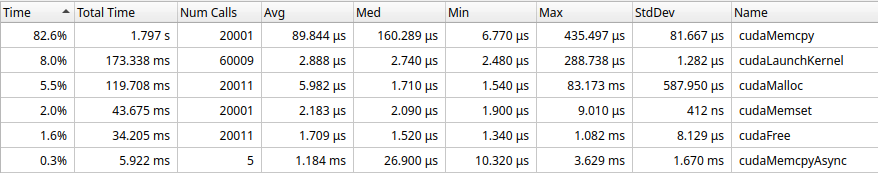
\includegraphics[scale=0.9]{images/cuda_api_summary.png}
\caption{Nsight Systems CUDA api summary}
\label{img:nsight_cuda_api}
\end{figure}

Figures \ref{img:nsight_1thread} and \ref{img:nsight_warp}
provide insights into the ratio of running times of different kernels.
It is apparent that the CSR matrix-vector dot product operation takes majority of the time.

\begin{figure}[H]
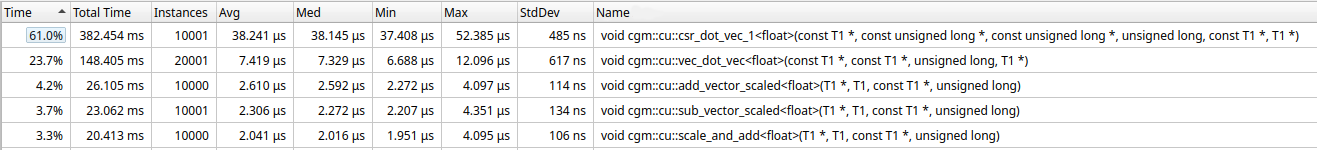
\includegraphics[scale=0.6]{images/csr1_kernel_summary.png}
\caption{One thread per row Nsight Systems kernel summary}
\label{img:nsight_1thread}
\end{figure}

\begin{figure}[H]
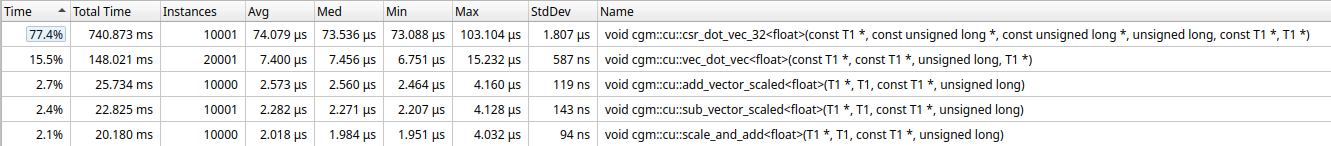
\includegraphics[scale=0.6]{images/csr32_kernel_summary.png}
\caption{One warp per row Nsight Systems kernel summary}
\label{img:nsight_warp}
\end{figure}

Further examining the CSR matrix-vector dot product kernel in NVIDIA Nsight compute,
we find that the launch parameters have sub-optimal occupancy as depicted in Figure \ref{img:nsys_occupancy}.
By launching 512 thread blocks instead of 1024 thread blocks, we achieve full 48 SM occupancy for both
the single thread per row kernel with 35 registers and the one warp per row kernel with 40 registers.

\begin{figure}[H]
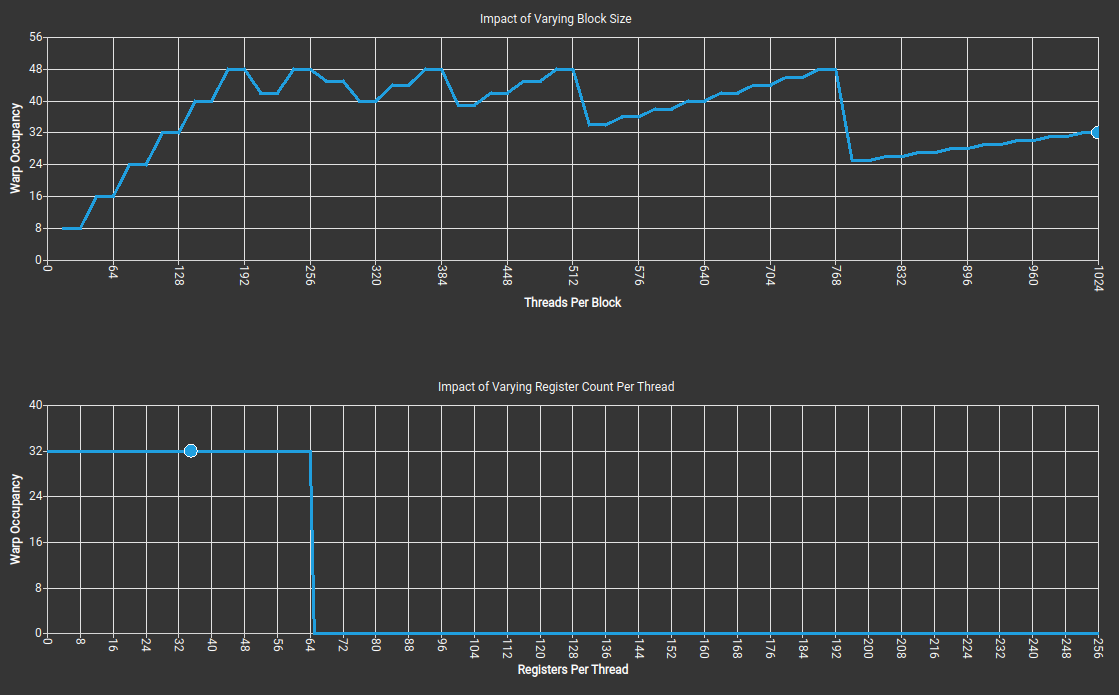
\includegraphics[scale=0.7]{images/csr_warp_occupancy.png}
\caption{CSR matrix-vector multiplication occupancy}
\label{img:nsys_occupancy}
\end{figure}

Upon analyzing the warp stall sampling in \ref{img:csr_stalling},
it becomes evident that the majority of time spent within the kernel is attributed to global memory access,
which proves to be challenging to optimize due to the inherent characteristics of the algorithm.
This kernel was launched with one warp per row and no stride,
Launching the kernel with fewer blocks and changing the jumps by 'warpCount'
to jumps by one may improve memory loads by hitting the cache.

\begin{figure}[H]
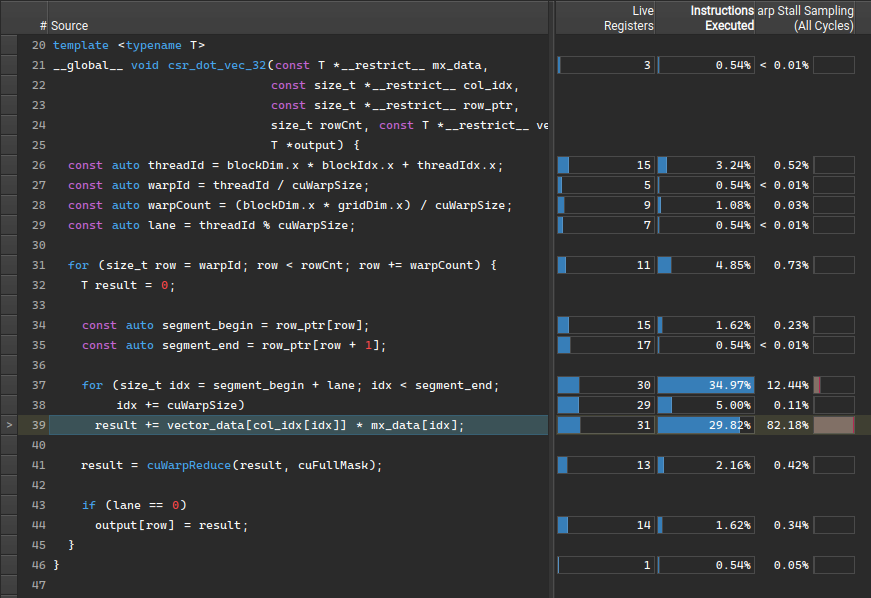
\includegraphics[scale=0.9]{images/csr_stalling.png}
\caption{CSR matrix-vector multiplication code statistics}
\label{img:csr_stalling}
\end{figure}

\section{Benchmarking}
The benchmarking was done on a Ryzen 5600x with 6 cores and 12 threads and an NVIDIA RTX 3700 Ti.
Only the 32bit float pipeline was utilized, 64 bit code was not benchmarked.

The code was benchmarked on 13 matrices of varying sizes and number of non-zero elements
from the SuiteSparse Matrix Collection \footnote{https://sparse.tamu.edu/}.
The matrix sizes ranged from ~7.000 to 1.200.000,
and the per-row mean non-zero element count ranged from 2 to 200.
Each calculation was ran 10 times per implementation tested.

The benchmarking started with the OpenMP parallelized version to establish a baseline,
followed by testing the CUDA accelerated version with one thread per matrix row,
which yielded unsatisfactory results.
Finally, the version with one warp per row was implemented and tested,
which showed significantly improved performance.
Unsurprisingly, it was found that each version was better suited for matrices with different sparsity.

The Figure \ref{img:speedup_size} shows the algorithm speedup depending on the matrix size,
showing the suitable kernel does not depend on the size of the matrix.
Figure \ref{img:speedup_nnz} shows the algorithm speedup depending on the mean amount of nonzero elements per row.

While testing, it was found that it is better to utilize the one thread per row kernel
when the mean number of nonzero elements is lower than ~8 and vice-versa, yielding the adaptive version.

\begin{figure}[H]
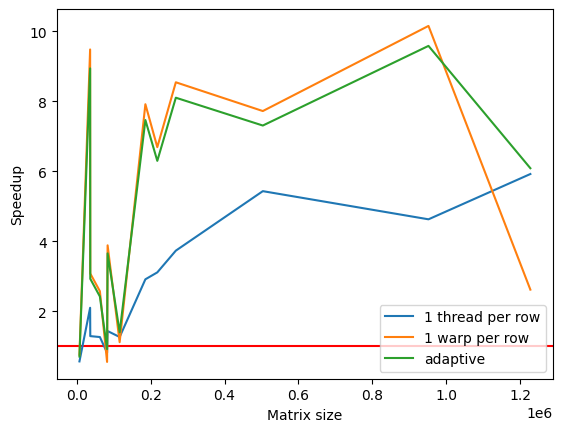
\includegraphics[]{images/speedup_size.png}
\centering
\caption{Speedup of the CUDA accelerated version depending on the matrix size}
\label{img:speedup_size}
\end{figure}

\begin{figure}[H]
\centering
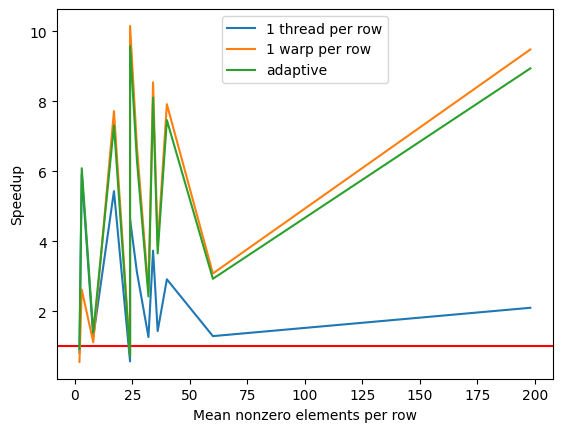
\includegraphics[]{images/speedup_nnz.png}
\caption{Speedup of the CUDA accelerated version depending on the mean number of non-zero elements per row}
\label{img:speedup_nnz}
\end{figure}

\bibliography{citations} 
\bibliographystyle{ieeetr}

\end{document}
